% !TEX root = report.tex

\section{Results}
\label{sec:results}
% Dazzling numerical results

\subsection{Attention weights}

\subsubsection{Attention model}

Show attention weights for Att model

% ATT_ct02_dr01_ks01_lu01_qt05_dw01_opa1_lr03_bs02_en02_dsaug07_wLTnum_LTnum_train_data
\begin{figure*}[t!]
    \centering
    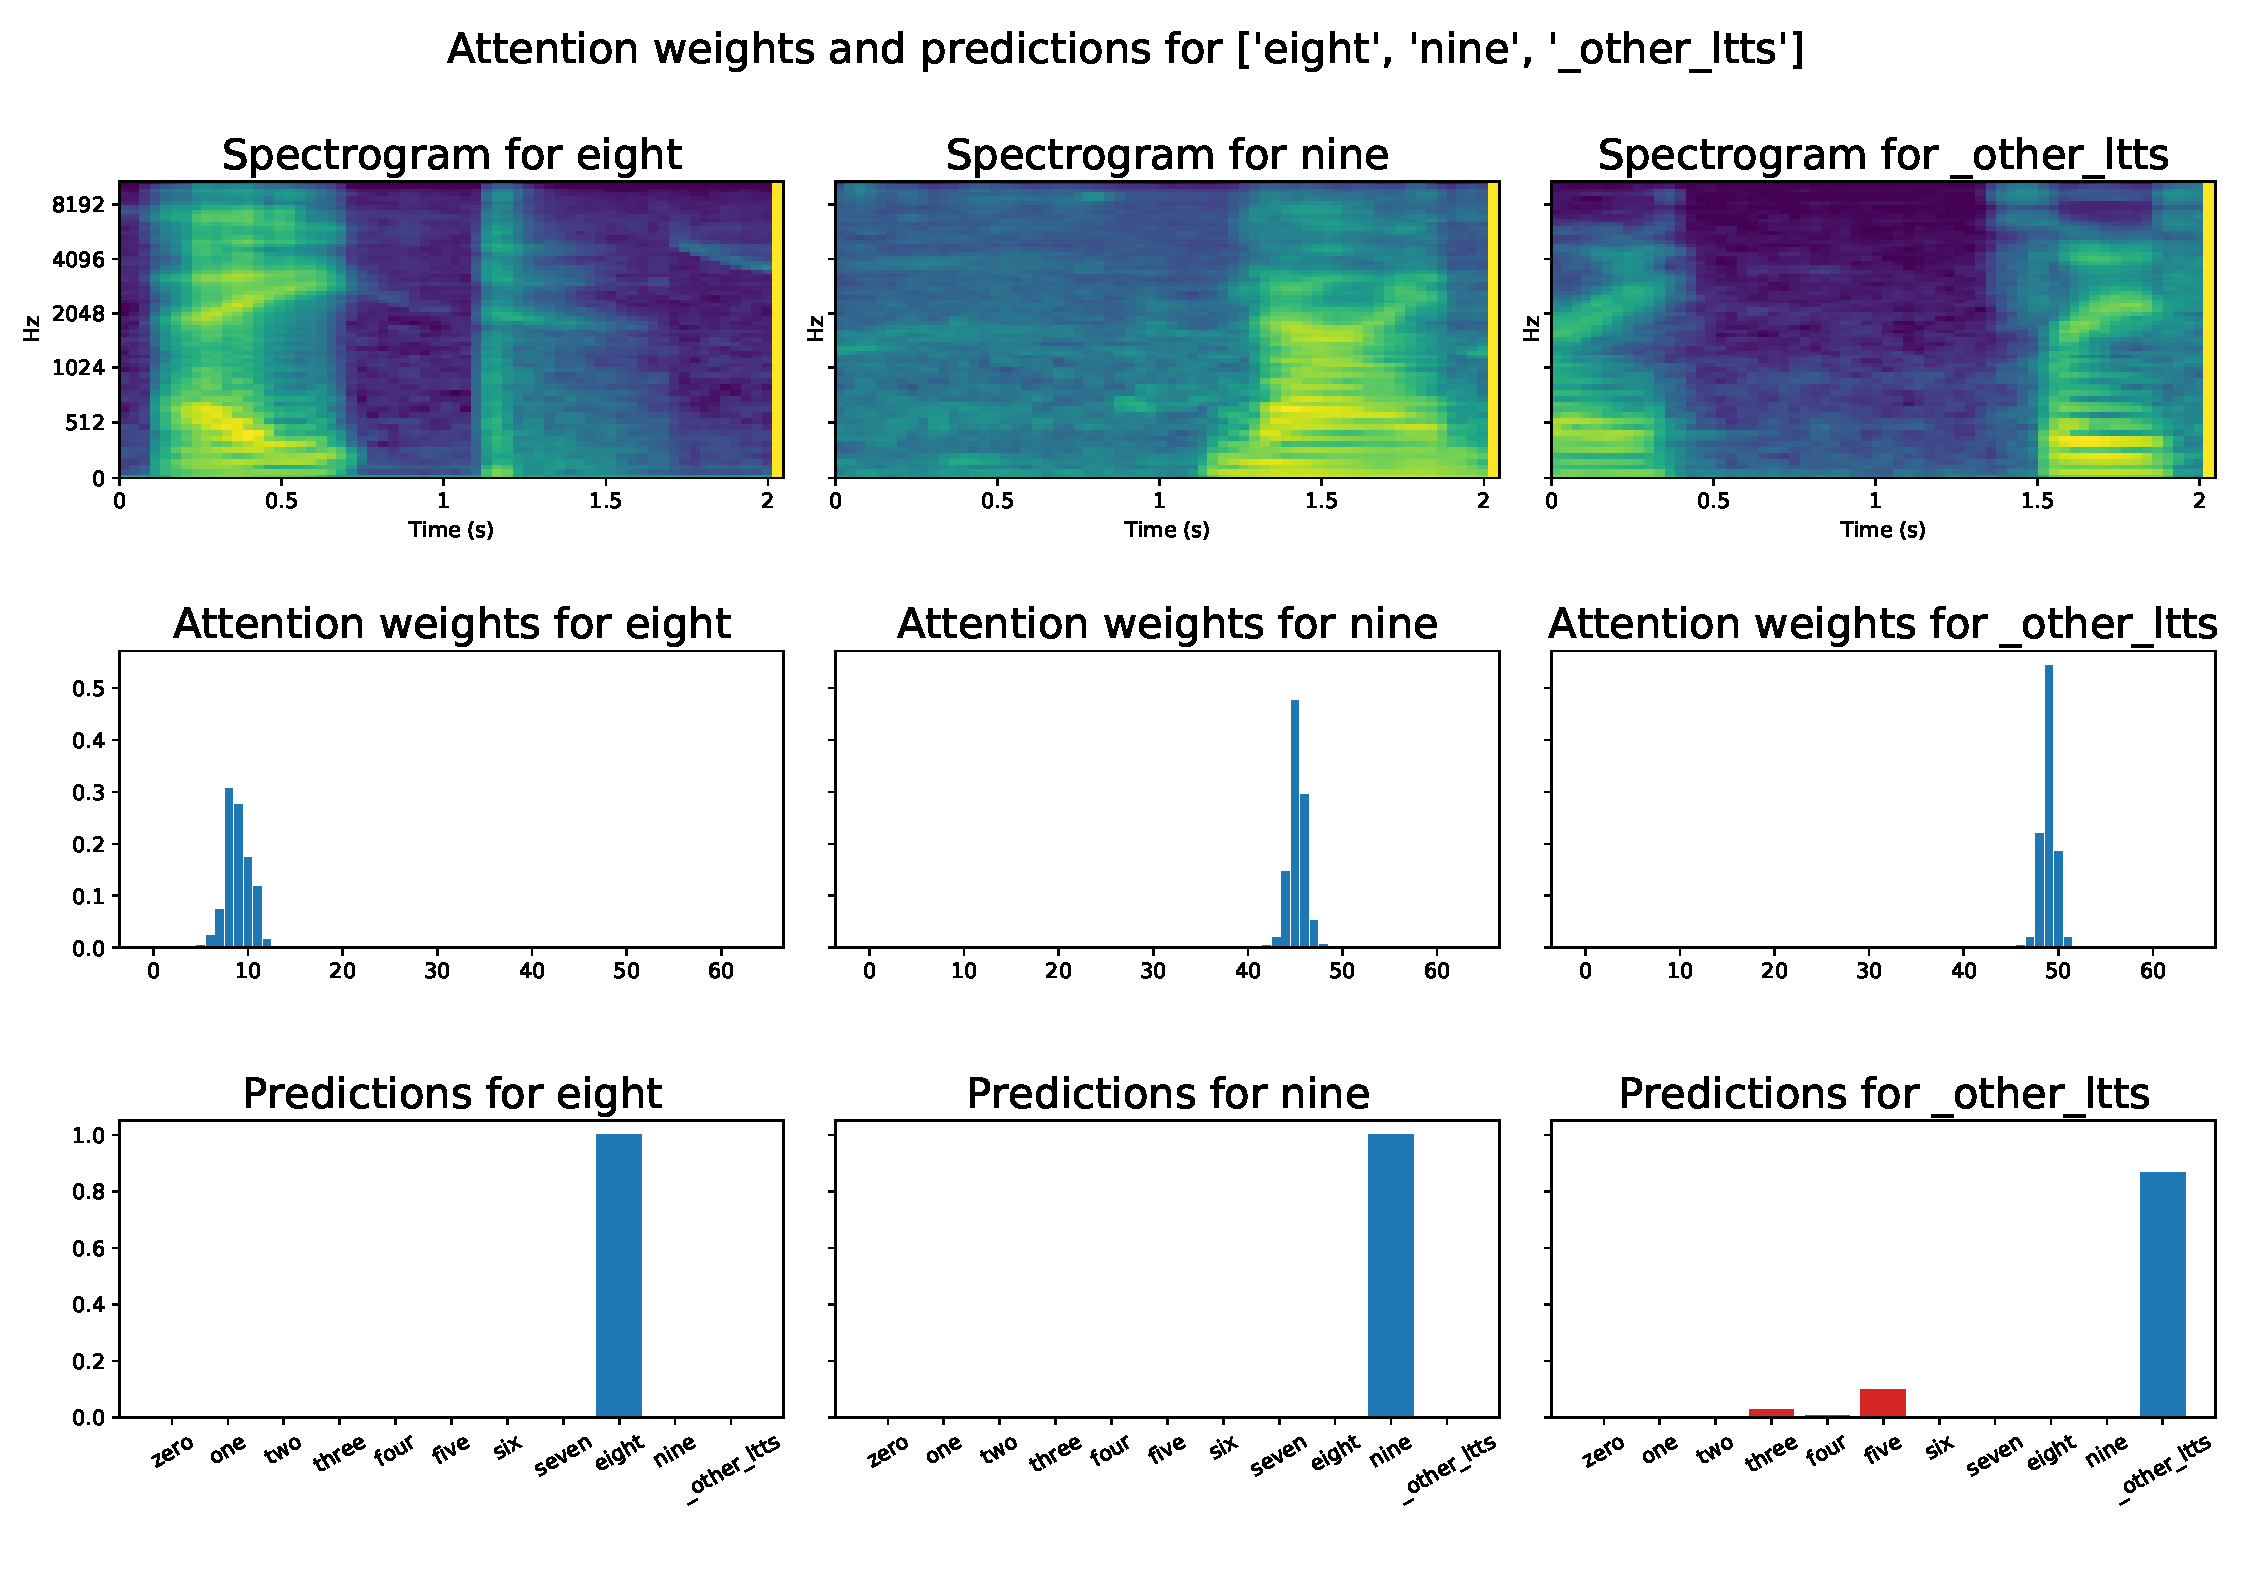
\includegraphics[width=0.9\linewidth]{ATT_ct02_dr01_ks01_lu01_qt05_dw01_opa1_lr03_bs02_en02_dsaug07_wLTnum_LTnum_train_data.pdf}
    \caption{Spectrograms, attention weights and predictions for three sample words.
    Notice how the attention weights correctly selected the interesting part of
    the ``eight'' spectrogram, avoiding the noise in the latter part.
    For ``\_other\_ltts'', which corresponds to a random audio snippet from the LibriTTS
    dataset, the attention weights still selected the section where a word is spoken,
    and, with some small uncertainty, the word is indeed recognized as ``other''.}%
    \label{fig:attention_weights_standard}
\end{figure*}

\subsubsection{AreaNet}

Show AreaNet

Show VerticalAreaNet

\subsection{Hyper-parameter analysis: CNN}

% \subsection{Hyper-parameter analysis}
% Hypa comparison
% First specific hypas

Tell total number of experiment per type

\subsection{Hyper-parameter analysis: Transfer}

\subsection{Hyper-parameter analysis: Attention}

Group by (conv, dropout, kernel, lstm, dense) to show difference in architecture

Group by query

Group by (lr, batch, epoch)

Group by dataset: not augmented, augmented

Group by type of augmentation: along both, one, none axis

Group by dataset: 1 sec vs loud section

\subsection{Architecture comparison}

Show best and top 5 average

Then aggregate table for cross architecture

Pick the best 5 models per category

Compare: CNN, Dense, Xception, EfficientB047, AreaNet, SimpleNet,
VerticalAreaNet on num, all, LTnum, LTall, numLS, allLS

Not every combination of everything

Show confusion matrices, speak about similar sounding words, note how AreaNet
does not miss them

\subsection{Stream predictions}

Compare normal vs loud

Attention vs Simple vs AreaNet vs VerticalAreaNet

Compare inference time, model size
